\subsection{\en{Thread Affinity}}
\subparagraph{}
\emph{\en{Thread Affinity}} είναι μια έννοια που περιλαμβάνει την βελτιστοποίηση του χρόνου εκτέλεσης ενός προγράμματος, μέσω βελτιστοποιήσεων στο εύρος ζώνης μνήμης, την αποφυγή καθυστέρησης μνήμης ή της  καθυστέρησης χρήσης προσωρινής μνήμης.

To \emph{\en{OpenMP 4.0}} εισάγει ένα σύνολο οδηγιών για την υποστήριξη του \emph{\en{thread affinity}}\cite{thread_affinity}. Η πλειοψηφία πλέον των μηχανημάτων βασίζονται στην \emph{\en{cc-NUMA}} αρχιτεκτονική. Ο λόγος που αυτό το σύστημα μνήμης έγινε κυρίαρχο, είναι η συνεχής αύξηση του αριθμού των επεξεργαστών. Η μονολιθική διασύνδεση μνήμης με σταθερό εύρος ζώνης μνήμης θα αποτελούσε πρόβλημα στην ραγδαία αύξηση των επεξεργαστών.

Στη \emph{\en{cc-NUMA}} αρχιτεκτονική κάθε υποδοχή συνδέεται με ένα υποσύνολο της συνολικής μνήμης του συστήματος. Μία διασύνδεση ενώνει τα υποσύνολα μεταξύ τους και δημιουργεί την εικόνα ενιαιας μνήμης στον χρήστη. Ενα τέτοιο σύστημα είναι ευκολότερο να επεκταθεί.

Το πλεονέκτημα της διασύνδεσης είναι ότι η εφαρμογή έχει πρόσβαση σε όλη την μνήμη του συστήματος, ανεξάρτητα από το που βρίσκονται τα δεδομένα. Ωστόσο, πλεον ο χρόνος πρόσβασης σε αυτά δεν ειναι ο σταθερός καθώς εξαρτάται από τη θέση τους στη μνήμη.


\begin{figure}[h]
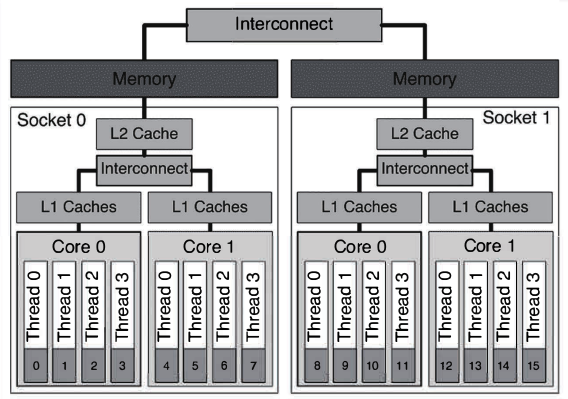
\includegraphics[width=0.75\textwidth]{numa}
\centering
\captionsetup{justification=centering, singlelinecheck=false}
	\caption{Αρχιτεκτονική \en{cc-NUMA}\cite{thenextstep152}}
\label{fig:numa}
\end{figure}

\clearpage{}
\subsubsection{\emph{\en{Thread affinity}} στο \emph{\en{OpenMP 4.0}}}
\subparagraph{}
Με το \emph{\en{thread affinity}} μπορεί να αποτραπεί η μετάβαση μιας διαδικασίας \emph{\en{MPI}} ή ενός νήματος του \emph{\en{OpenMP}} σε απομακρυσμένο υλικό.
Η μετάβαση αυτή θα μπορούσε να προκαλέσει μείωση της απόδοσης του κώδικα. Η έκδοση 4.0 του \emph{\en{OpenMP}} εισήγαγε ρυθμίσεις για το χειρισμό του \emph{\en{affinity}} μέσω των μεταβλητών περιβάλλοντος  \emph{\en{OMP\_PLACES}} και \emph{\en{OMP\_PROC\_BIND}}\cite{affinity1}.
\ \\
\ \\
\paragraph{\emph{\en{Thread Binding}}}
\subparagraph{}
Οι προαναφερθήσες μεταβλητές, μπορούν να καθορίσουν σε θέση στο υλικό θα ανατεθούν τα νήματα μια ομάδας, που δημιουργήθηκε για να εκτελέσει μια διεργασία.
\ \\
\ \\
\textbf{Παράδειγμα}: Αν υπάρχουν δύο \emph{\en{sockets}} και ορισθεί $$OMP\_PLACES=sockets$$, τότε:
\begin{itemize}
\item{το νήμα 0 θα πάει στο \emph{\en{socket} 0}}
\item{το νήμα 1 θα πάει στο \emph{\en{socket} 1}}
\item{το νήμα 2 θα πάει στο \emph{\en{socket} 2}} κοκ.
\end{itemize}

Επίσης, αν δυο \emph{\en{socket}} έχουν συνολικά 16 πυρήνες και ο χρήστης ορίσει $$OMP\_PLACES=cores$$ \begin{center}και\end{center} $$OMP\_PROC\_BIND=close$$ τότε:
\begin{itemize}
\item{το νήμα 0	θα πάει στον πυρήνα 0 που βρίσκεται στο \emph{\en{socket}} 0}
\item{το νήμα 1	θα πάει στον πυρήνα 1 που βρίσκεται στο \emph{\en{socket}} 0}
\item{το νήμα 2	θα πάει στον πυρήνα 2 που βρίσκεται στο \emph{\en{socket}} 0}
\item{...}
\item{το νήμα 7 στον πυρήνα 7 του \emph{\en{socket}} 0}
\item{το νήμα 8 στον πυρήνα 8 του \emph{\en{socket}} 1, κλπ}
\end{itemize}

\clearpage
Το όρισμα \emph{\en{OMP\_PROC\_BIND}} ορίζει τον τρόπο με τον οποίο τα νήματα ανατίθεvται στους πόρους. Η επιλογή \emph{\en{OMP\_PROC\_BIND = close}} σημαίνει ότι η ανάθεση περνά διαδοχικά στις διαθέσιμες θέσεις. Μια αλλη αποδεκτή τιμή για το \emph{\en{OMP\_PROC\_BIND}} είναι η \emph{\en{spread}}. Η λειτουργία της φαίνεται στο παρακάτω παράδειγμα:
\ \\
\textbf{Παράδειγμα}, για:
$$OMP\_PLACES=cores$$
$$OMP\_PROC\_BIND=spread$$

\begin{itemize}
\item{το νήμα 0 πάει στον πυρήνα 0, που βρίσκεται στο \emph{\en{socket}} 0}
\item{το νήμα 1 πάει στον πυρήνα 8, που βρίσκεται στο \emph{\en{socket}} 1}
\item{το νήμα 2 πάει στον πυρήνα 1, που βρίσκεται στο \emph{\en{socket}} 0}
\item{...}
\item{το νήμα 15 πάει στον πυρήνα 15, που βρίσκεται στο \emph{\en{socket}} 1}
\end{itemize}

Η επιλογή \emph{\en{OMP\_PROC\_BIND=master}} αναθέται τα νήματα στο ίδιο σημείο που είναι και το κύριο νήμα της ομάδας. Αυτή η επιλογή χρησιμοποιείται όταν δημιουργούνται πολλές ομάδες αναδρομικά.

Εκτός από τις επιλογές \emph{\en{cores}} και \emph{\en{sockets}} για τη μεταβλητή \emph{\en{OMP\_PLACES}}, υπάρχει και η \emph{\en{threads}} που χρησιμοποιείται σε ειδικές περιπτώσεις αρχιτεκτονικής, δηλαδή σε περιπτώσεις που οι επεξεργαστές περιέχουν νήματα\cite{affinity2}.

\ \\
\ \\
\subsubsection{Το \emph{\en{thread affinity}} στην πράξη}
\subparagraph{}
Δυστυχώς, δεν υπάρχει καμία καλύτερη επιλογή για τη ρύθμιση της τοποθέτησης νήματος και της συγγένειας. Η επιλογή εξαρτάται από την εκάστοτε εφαρμογή που πρόκειται να εκτελεστεί. Ακόμη, ο χρήστης θα πρέπει να λαμβάνει υπόψη τις εξής παραμέτρους\cite{affinity3}:
\begin{itemize}
\item{Οι χρόνοι εκτέλεσης μιας εργασίας μπορούν να επηρεαστούν από άλλες εργασίες που εκτελούνται στο ίδιο μηχάνημα εκείνη τη στιγμή και μοιράζονται πρόσβαση στο δίκτυο, τον δίαυλο μνήμης και στην προσωρινή μνήμη.}
\item{Το λειτουργικό σύστημα ενός μηχανήματος, εκτελεί ταυτόχρονα τις δικές του διεργασίες}
\end{itemize}